\documentclass[12pt,a4paper]{article}
\usepackage[utf8]{inputenc}
\usepackage[german]{babel}
\usepackage[T1]{fontenc}
\usepackage{amsmath}
\usepackage{amsfonts}
\usepackage{amssymb}
\usepackage{graphicx}
\usepackage{siunitx}
\usepackage[left=2cm,right=2cm,top=2cm,bottom=2cm]{geometry}
\author{Tim}

\begin{document}
\setlength{\parindent}{0pt} 
\begin{center}
{\LARGE Versuchsprotokoll}\\
\begin{large}
zum Grundpraktikum Physik Teil II\\[0.4cm]
an der RWTH Aachen\\
I. Physikalisches Institut B\\[4.5cm]
\Large\textbf{\textsl{Optik II}}\\[4cm]
\normalsize\textit{vorgelegt\\von}\\[0.4cm]
\large{Moritz Berger\\Tim Herbermann\\Gerald Kolter\\Sebastian Siebert}\\[1cm]
\large \textit{Gruppe A07} \\ [3cm]
\large \textbf{Sommersemester 2017}
\end{large}
\end{center}
\newpage

\tableofcontents
\newpage

\section{Grundlagen}

Im folgenden Versuch soll mithilfe eines Michelson-Interferometers die Wellenlänge eines Lasers bestimmt werden. Anschließend soll die Druckabhängigkeit des Brechungsindex von Luft untersucht werden. Als letztes wird der Brechungsindex von $\text{CO}_2$ bestimmt.\\
\\
Grundlage des Versuches ist  die Interferenz eines kohärenten Wellenzuges mit sich selbst durch Amlitudenaufspaltung. Die dadurch entstehenden Teilstrahlen durchlaufen eine unterschiedliche Strecke, bis sie wieder vereinigt werden. Dadurch besitzen sie eine feste Phasenbeziehung zueinander und sind somit kohärent und damit interferenzfähig.\\
Beim Michelson-Interferometer wird ein leicht divergenter Strahl verwendet. Dadurch gibt es für unterschiedliche Divergenzwinkel $\theta$ andere Phasenverschiebungen, da die Strecke mit $\cos(\theta)$ modifiziert wird. Für den Streckenunterschied gilt dann:
\begin{equation}
\delta = \dfrac{2\pi}{\lambda} \cdot 2d \cos(\theta)
\end{equation}
Betrachtet man Interferenzmaxima muss $\delta = 2\pi m$, $m=0,1,2,...$, gelten und damit:
\begin{equation}
2d \cos(\theta) = m\lambda
\label{equ:Maxima}
\end{equation}

Durch Taylorentwicklung ergibt sich als lineare Näherung für die Druckabhängigkeit des Brechungsindexes vom Druck die Formel:

\begin{equation}
n(P) = 1+\frac{\Delta n}{\Delta P} \cdot P
\label{eq:DruckBrechzahl}
\end{equation}

Aus der optischen Wegdifferenz und der Maximumsbedingung ergibt sich somit der Zusammenhang:

\begin{equation}
\frac{\Delta n}{\Delta P} = \frac{\Delta m}{\Delta P} \cdot  \frac{\lambda}{2L}
\label{equ:DruckBrechung}
\end{equation}

Ähnliche Überlegungen ergeben für den Brechungsindex von $CO_2$ führen zu den Zusammenhängen

\begin{equation}
n_{CO_2} = n_{Luft} + \Delta n
\label{eq:COO_n}
\end{equation}

wobei gilt

\begin{equation}
\Delta n = \Delta m \frac{\lambda}{2L}
\label{eq:COO_dn}
\end{equation}



\section{Aufbau und Durchführung}

\begin{figure}
\centering
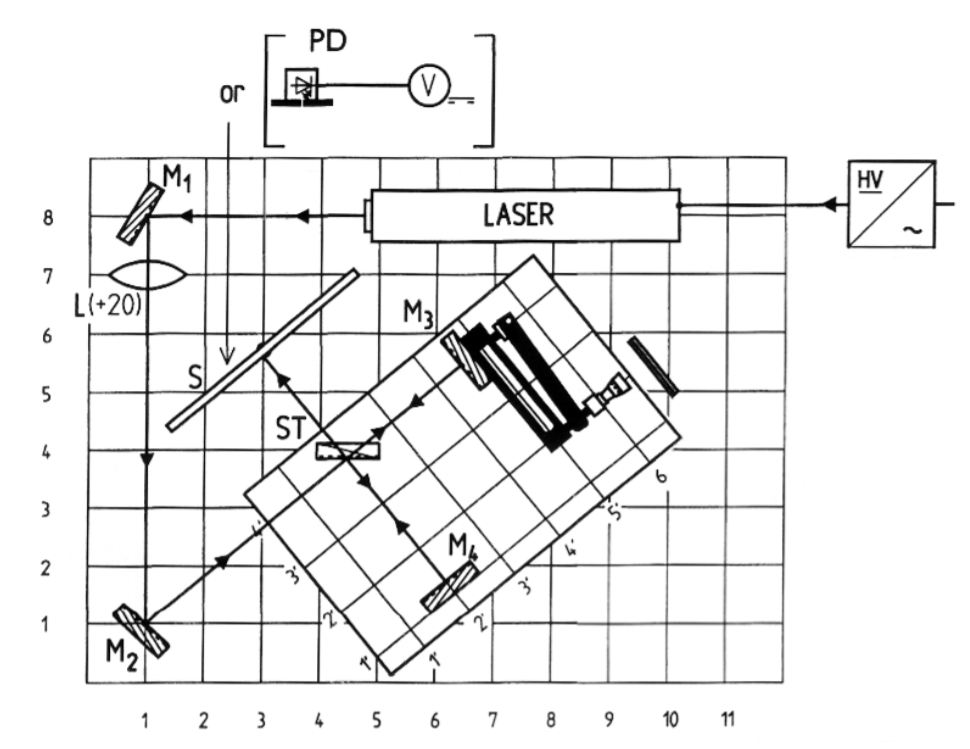
\includegraphics[scale=0.6]{Bilder/Aufbau}
\caption{Aufbau eines Michelson-Interferometers}
\label{fig:Aufbau}
\end{figure}

Zu Beginn wird die Wellenlänge des grünen Lasers durch Veränderung der optischen Weglänge bestimmt. Eine Skizze des Versuchsaufbaus ist in Abbildung \ref{fig:Aufbau} gezeigt.
Dazu wird der Spiegel M3 verschoben, wobei im Interferenzbild am Schirm aufgrund der Veränderung der optischen Weglänge nacheinander im Zentrum Maxima verschwinden bzw. erscheinen. Eine Wechsel von $\Delta m$ Maxima entspricht dann einer gewissen Verschiebung $\Delta d$. Die Wellenlänge des Lasers 
ergibt sich dann aus Gleichung \ref{equ:Maxima} für $\theta = 0$.\\

Die Verschiebung von M3 erfolgt über einen Feintrieb. Es muss somit zuvor eine Kalibrierung zwischen (relativer) Spiegelposition $d$ und Feintriebskala $s$ vorgenommen werden. Dafür wird ein roter He-Ne-Laser mit bekannter Wellenlänge ($\lambda = 632,8$ nm) verwendet.\\

Zur Bestimmung der Druckabhängigkeit des Brechungsindexes von Luft wird eine Glasparzelle in den Strahlengang zwischen Strahlteiler ST und Spiegel M3 eingebracht. Der veränderte Aufbau ist in Abbildung \ref{fig:AufbauDruck} dargestellt.

\begin{figure}
\begin{center}
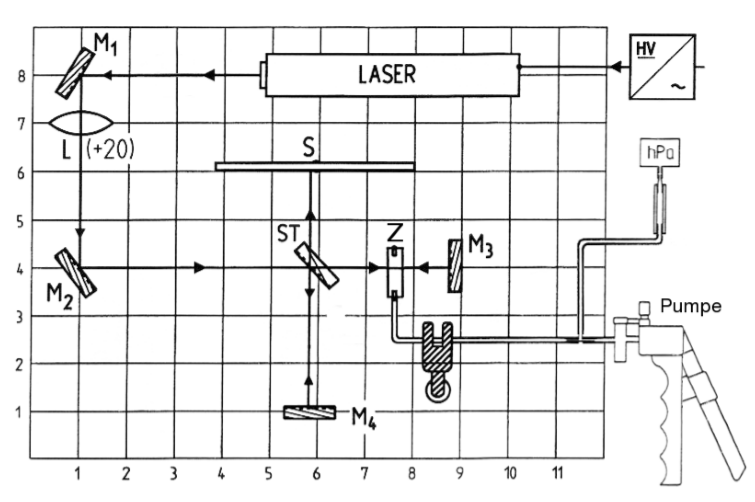
\includegraphics[scale=0.6]{Bilder/AufbauDruck.png}
\caption{Aufbau zur Bestimmung der Druckabhängigkeit des Brechungsindex. (Quelle: Praktikumsskript S.41)}
\label{fig:AufbauDruck}
\end{center}
\end{figure}

Mit der Handpumpe wird der Druck in der Parzelle solange verringert, bis auf dem Schirm ein vollständiger Wechsel von Maximum zu Maximum durchlaufen wurde. Für jeden dieser Schritte wird der Druck gemessen und notiert. Die Druckabhängigkeit ergibt sich dann mithilfe von Gleichung \ref{equ:DruckBrechung}.

\section{Auswertung}

\subsection{Kalibration}

\subsection{Bestimmung der Wellenlänge}

\subsection{Druckabhängigkeit des Brechungsindex}

\subsection{Brechungsindex von Kohlenstoffdioxid}
In diesem Teilsversuch sollte mithilfe der Resultate von den vorherigen Versuchen der Brechungsindex von $CO_2$ bestimmt werden. Dabei wird zuerst nach Gleichung \ref{eq:COO_dn} der Unterschied im Brechungsindex von Luft und $CO_2$ bestimmt. Dazu werden, wie in den Versuchen vorher, wieder die Anzahl der durchlaufenen Interferenzmaxima beim füllen der Parzelle mit $CO_2$ gemessen. Die Resultate sind in Tabelle \ref{tab:COO_Rohdaten} aufgelistet.

\begin{table}
\center
\begin{tabular}{|c|c|c|c|c|c|c|c|c|}
\hline
Messung & 1 & 2 & 3 & 4 & 5 & 6 & 7 & 8\\
\hline
$\Delta m$ & 5.1 & 4.8 & 5.0 & 4.9 & 4.7 & 5.1 & 5.0 & 4.8\\
\hline
\end{tabular}
\caption{Rohdaten der durchlaufenen Interferenzmaxima. Nach der Bestimmung der ungefähren durchläufe wurde noch abgeschätzt, um welchen Anteil Anfangs- und Endbild verschoben sind.}
\label{tab:COO_Rohdaten}
\end{table}

Hieraus wurde der Mittelwert mitsamt seiner Standardabweichung gebildet:
\begin{equation}
\Delta m = 4.92 \pm 0.15
\end{equation}
Daraus wird mittels Gleichung \ref{eq:COO_dn} der Unterschied im Brechungsindex bestimmt:
\begin{equation}
\Delta n = (1.287 \pm 0.039 \pm 0.015)\cdot 10^{-4}
\end{equation}
Der statistische Fehler Bestimmt sich alllein durch die Mehrfachmessung.
Der Systematische Fehler besteht aus den quadratisch addierten Fehlern auf der Wellenlänge aus dem Vorversuch und aus dem Fehler auf der Länge L, der hier mit 1\% angenommen wird:
\begin{equation}
\sigma_{stat} = \dfrac{\Delta n}{\Delta m} \cdot \sigma_{\Delta m}
\end{equation}
\begin{equation}
\sigma_{sys} = \sqrt{\left(\dfrac{\Delta n}{\lambda} \cdot \sigma_{\lambda}\right)^2 + \left(\dfrac{\Delta n}{L} \cdot \sigma_{L}\right)^2}
\end{equation}

Um aus diesem Ergebnis nun den Brechungsindex von $CO_2$ zu bestimmen wird Gleichung \ref{eq:COO_n} benutzt. Dafür wird allerdings zuerst der Brechungsindex von Luft mithilfe der Resultate von Kapitel 3.3 und Gleichung \ref{eq:DruckBrechzahl} bestimmt. Dabei wird der Umgebungsdruck mit 979 hPa angenommen:
\begin{equation}
n_{Luft}-1 = (2.56 \pm 0.03)\cdot 10^{-4}
\end{equation}
Daraus folgt dann der Brechungsindex von $CO_2$:
\begin{equation}
n_{CO_2}-1 = (3.84 \pm 0.04 \pm 0.03)\cdot 10^{-4}
\end{equation}

\paragraph{Zwischenfazit}


\section{Fazit}

\end{document}
